\documentclass[crop=false,class=book]{standalone}
%---------------PREAMBLE------------%
%---------------------------Packages----------------------------%
\usepackage{geometry}
\geometry{b5paper, margin=1.0in}
\usepackage[T1]{fontenc}
\usepackage{graphicx, float}            % Graphics/Images.
\usepackage{natbib}                     % For bibliographies.
\bibliographystyle{agsm}                % Bibliography style.
\usepackage[french, english]{babel}     % Language typesetting.
\usepackage[dvipsnames]{xcolor}         % Color names.
\usepackage{listings}                   % Verbatim-Like Tools.
\usepackage{mathtools, esint, mathrsfs} % amsmath and integrals.
\usepackage{amsthm, amsfonts, amssymb}  % Fonts and theorems.
\usepackage{tcolorbox}                  % Frames around theorems.
\usepackage{upgreek}                    % Non-Italic Greek.
\usepackage{fmtcount, etoolbox}         % For the \book{} command.
\usepackage[newparttoc]{titlesec}       % Formatting chapter, etc.
\usepackage{titletoc}                   % Allows \book in toc.
\usepackage[nottoc]{tocbibind}          % Bibliography in toc.
\usepackage[titles]{tocloft}            % ToC formatting.
\usepackage{pgfplots, tikz}             % Drawing/graphing tools.
\usepackage{imakeidx}                   % Used for index.
\usetikzlibrary{
    calc,                   % Calculating right angles and more.
    angles,                 % Drawing angles within triangles.
    arrows.meta,            % Latex and Stealth arrows.
    quotes,                 % Adding labels to angles.
    positioning,            % Relative positioning of nodes.
    decorations.markings,   % Adding arrows in the middle of a line.
    patterns,
    arrows
}                                       % Libraries for tikz.
\pgfplotsset{compat=1.9}                % Version of pgfplots.
\usepackage[font=scriptsize,
            labelformat=simple,
            labelsep=colon]{subcaption} % Subfigure captions.
\usepackage[font={scriptsize},
            hypcap=true,
            labelsep=colon]{caption}    % Figure captions.
\usepackage[pdftex,
            pdfauthor={Ryan Maguire},
            pdftitle={Mathematics and Physics},
            pdfsubject={Mathematics, Physics, Science},
            pdfkeywords={Mathematics, Physics, Computer Science, Biology},
            pdfproducer={LaTeX},
            pdfcreator={pdflatex}]{hyperref}
\hypersetup{
    colorlinks=true,
    linkcolor=blue,
    filecolor=magenta,
    urlcolor=Cerulean,
    citecolor=SkyBlue
}                           % Colors for hyperref.
\usepackage[toc,acronym,nogroupskip,nopostdot]{glossaries}
\usepackage{glossary-mcols}
%------------------------Theorem Styles-------------------------%
\theoremstyle{plain}
\newtheorem{theorem}{Theorem}[section]

% Define theorem style for default spacing and normal font.
\newtheoremstyle{normal}
    {\topsep}               % Amount of space above the theorem.
    {\topsep}               % Amount of space below the theorem.
    {}                      % Font used for body of theorem.
    {}                      % Measure of space to indent.
    {\bfseries}             % Font of the header of the theorem.
    {}                      % Punctuation between head and body.
    {.5em}                  % Space after theorem head.
    {}

% Italic header environment.
\newtheoremstyle{thmit}{\topsep}{\topsep}{}{}{\itshape}{}{0.5em}{}

% Define environments with italic headers.
\theoremstyle{thmit}
\newtheorem*{solution}{Solution}

% Define default environments.
\theoremstyle{normal}
\newtheorem{example}{Example}[section]
\newtheorem{definition}{Definition}[section]
\newtheorem{problem}{Problem}[section]

% Define framed environment.
\tcbuselibrary{most}
\newtcbtheorem[use counter*=theorem]{ftheorem}{Theorem}{%
    before=\par\vspace{2ex},
    boxsep=0.5\topsep,
    after=\par\vspace{2ex},
    colback=green!5,
    colframe=green!35!black,
    fonttitle=\bfseries\upshape%
}{thm}

\newtcbtheorem[auto counter, number within=section]{faxiom}{Axiom}{%
    before=\par\vspace{2ex},
    boxsep=0.5\topsep,
    after=\par\vspace{2ex},
    colback=Apricot!5,
    colframe=Apricot!35!black,
    fonttitle=\bfseries\upshape%
}{ax}

\newtcbtheorem[use counter*=definition]{fdefinition}{Definition}{%
    before=\par\vspace{2ex},
    boxsep=0.5\topsep,
    after=\par\vspace{2ex},
    colback=blue!5!white,
    colframe=blue!75!black,
    fonttitle=\bfseries\upshape%
}{def}

\newtcbtheorem[use counter*=example]{fexample}{Example}{%
    before=\par\vspace{2ex},
    boxsep=0.5\topsep,
    after=\par\vspace{2ex},
    colback=red!5!white,
    colframe=red!75!black,
    fonttitle=\bfseries\upshape%
}{ex}

\newtcbtheorem[auto counter, number within=section]{fnotation}{Notation}{%
    before=\par\vspace{2ex},
    boxsep=0.5\topsep,
    after=\par\vspace{2ex},
    colback=SeaGreen!5!white,
    colframe=SeaGreen!75!black,
    fonttitle=\bfseries\upshape%
}{not}

\newtcbtheorem[use counter*=remark]{fremark}{Remark}{%
    fonttitle=\bfseries\upshape,
    colback=Goldenrod!5!white,
    colframe=Goldenrod!75!black}{ex}

\newenvironment{bproof}{\textit{Proof.}}{\hfill$\square$}
\tcolorboxenvironment{bproof}{%
    blanker,
    breakable,
    left=3mm,
    before skip=5pt,
    after skip=10pt,
    borderline west={0.6mm}{0pt}{green!80!black}
}

\AtEndEnvironment{lexample}{$\hfill\textcolor{red}{\blacksquare}$}
\newtcbtheorem[use counter*=example]{lexample}{Example}{%
    empty,
    title={Example~\theexample},
    boxed title style={%
        empty,
        size=minimal,
        toprule=2pt,
        top=0.5\topsep,
    },
    coltitle=red,
    fonttitle=\bfseries,
    parbox=false,
    boxsep=0pt,
    before=\par\vspace{2ex},
    left=0pt,
    right=0pt,
    top=3ex,
    bottom=1ex,
    before=\par\vspace{2ex},
    after=\par\vspace{2ex},
    breakable,
    pad at break*=0mm,
    vfill before first,
    overlay unbroken={%
        \draw[red, line width=2pt]
            ([yshift=-1.2ex]title.south-|frame.west) to
            ([yshift=-1.2ex]title.south-|frame.east);
        },
    overlay first={%
        \draw[red, line width=2pt]
            ([yshift=-1.2ex]title.south-|frame.west) to
            ([yshift=-1.2ex]title.south-|frame.east);
    },
}{ex}

\AtEndEnvironment{ldefinition}{$\hfill\textcolor{Blue}{\blacksquare}$}
\newtcbtheorem[use counter*=definition]{ldefinition}{Definition}{%
    empty,
    title={Definition~\thedefinition:~{#1}},
    boxed title style={%
        empty,
        size=minimal,
        toprule=2pt,
        top=0.5\topsep,
    },
    coltitle=Blue,
    fonttitle=\bfseries,
    parbox=false,
    boxsep=0pt,
    before=\par\vspace{2ex},
    left=0pt,
    right=0pt,
    top=3ex,
    bottom=0pt,
    before=\par\vspace{2ex},
    after=\par\vspace{1ex},
    breakable,
    pad at break*=0mm,
    vfill before first,
    overlay unbroken={%
        \draw[Blue, line width=2pt]
            ([yshift=-1.2ex]title.south-|frame.west) to
            ([yshift=-1.2ex]title.south-|frame.east);
        },
    overlay first={%
        \draw[Blue, line width=2pt]
            ([yshift=-1.2ex]title.south-|frame.west) to
            ([yshift=-1.2ex]title.south-|frame.east);
    },
}{def}

\AtEndEnvironment{ltheorem}{$\hfill\textcolor{Green}{\blacksquare}$}
\newtcbtheorem[use counter*=theorem]{ltheorem}{Theorem}{%
    empty,
    title={Theorem~\thetheorem:~{#1}},
    boxed title style={%
        empty,
        size=minimal,
        toprule=2pt,
        top=0.5\topsep,
    },
    coltitle=Green,
    fonttitle=\bfseries,
    parbox=false,
    boxsep=0pt,
    before=\par\vspace{2ex},
    left=0pt,
    right=0pt,
    top=3ex,
    bottom=-1.5ex,
    breakable,
    pad at break*=0mm,
    vfill before first,
    overlay unbroken={%
        \draw[Green, line width=2pt]
            ([yshift=-1.2ex]title.south-|frame.west) to
            ([yshift=-1.2ex]title.south-|frame.east);},
    overlay first={%
        \draw[Green, line width=2pt]
            ([yshift=-1.2ex]title.south-|frame.west) to
            ([yshift=-1.2ex]title.south-|frame.east);
    }
}{thm}

%--------------------Declared Math Operators--------------------%
\DeclareMathOperator{\adjoint}{adj}         % Adjoint.
\DeclareMathOperator{\Card}{Card}           % Cardinality.
\DeclareMathOperator{\curl}{curl}           % Curl.
\DeclareMathOperator{\diam}{diam}           % Diameter.
\DeclareMathOperator{\dist}{dist}           % Distance.
\DeclareMathOperator{\Div}{div}             % Divergence.
\DeclareMathOperator{\Erf}{Erf}             % Error Function.
\DeclareMathOperator{\Erfc}{Erfc}           % Complementary Error Function.
\DeclareMathOperator{\Ext}{Ext}             % Exterior.
\DeclareMathOperator{\GCD}{GCD}             % Greatest common denominator.
\DeclareMathOperator{\grad}{grad}           % Gradient
\DeclareMathOperator{\Ima}{Im}              % Image.
\DeclareMathOperator{\Int}{Int}             % Interior.
\DeclareMathOperator{\LC}{LC}               % Leading coefficient.
\DeclareMathOperator{\LCM}{LCM}             % Least common multiple.
\DeclareMathOperator{\LM}{LM}               % Leading monomial.
\DeclareMathOperator{\LT}{LT}               % Leading term.
\DeclareMathOperator{\Mod}{mod}             % Modulus.
\DeclareMathOperator{\Mon}{Mon}             % Monomial.
\DeclareMathOperator{\multideg}{mutlideg}   % Multi-Degree (Graphs).
\DeclareMathOperator{\nul}{nul}             % Null space of operator.
\DeclareMathOperator{\Ord}{Ord}             % Ordinal of ordered set.
\DeclareMathOperator{\Prin}{Prin}           % Principal value.
\DeclareMathOperator{\proj}{proj}           % Projection.
\DeclareMathOperator{\Refl}{Refl}           % Reflection operator.
\DeclareMathOperator{\rk}{rk}               % Rank of operator.
\DeclareMathOperator{\sgn}{sgn}             % Sign of a number.
\DeclareMathOperator{\sinc}{sinc}           % Sinc function.
\DeclareMathOperator{\Span}{Span}           % Span of a set.
\DeclareMathOperator{\Spec}{Spec}           % Spectrum.
\DeclareMathOperator{\supp}{supp}           % Support
\DeclareMathOperator{\Tr}{Tr}               % Trace of matrix.
%--------------------Declared Math Symbols--------------------%
\DeclareMathSymbol{\minus}{\mathbin}{AMSa}{"39} % Unary minus sign.
%------------------------New Commands---------------------------%
\DeclarePairedDelimiter\norm{\lVert}{\rVert}
\DeclarePairedDelimiter\ceil{\lceil}{\rceil}
\DeclarePairedDelimiter\floor{\lfloor}{\rfloor}
\newcommand*\diff{\mathop{}\!\mathrm{d}}
\newcommand*\Diff[1]{\mathop{}\!\mathrm{d^#1}}
\renewcommand*{\glstextformat}[1]{\textcolor{RoyalBlue}{#1}}
\renewcommand{\glsnamefont}[1]{\textbf{#1}}
\renewcommand\labelitemii{$\circ$}
\renewcommand\thesubfigure{%
    \arabic{chapter}.\arabic{figure}.\arabic{subfigure}}
\addto\captionsenglish{\renewcommand{\figurename}{Fig.}}
\numberwithin{equation}{section}

\renewcommand{\vector}[1]{\boldsymbol{\mathrm{#1}}}

\newcommand{\uvector}[1]{\boldsymbol{\hat{\mathrm{#1}}}}
\newcommand{\topspace}[2][]{(#2,\tau_{#1})}
\newcommand{\measurespace}[2][]{(#2,\varSigma_{#1},\mu_{#1})}
\newcommand{\measurablespace}[2][]{(#2,\varSigma_{#1})}
\newcommand{\manifold}[2][]{(#2,\tau_{#1},\mathcal{A}_{#1})}
\newcommand{\tanspace}[2]{T_{#1}{#2}}
\newcommand{\cotanspace}[2]{T_{#1}^{*}{#2}}
\newcommand{\Ckspace}[3][\mathbb{R}]{C^{#2}(#3,#1)}
\newcommand{\funcspace}[2][\mathbb{R}]{\mathcal{F}(#2,#1)}
\newcommand{\smoothvecf}[1]{\mathfrak{X}(#1)}
\newcommand{\smoothonef}[1]{\mathfrak{X}^{*}(#1)}
\newcommand{\bracket}[2]{[#1,#2]}

%------------------------Book Command---------------------------%
\makeatletter
\renewcommand\@pnumwidth{1cm}
\newcounter{book}
\renewcommand\thebook{\@Roman\c@book}
\newcommand\book{%
    \if@openright
        \cleardoublepage
    \else
        \clearpage
    \fi
    \thispagestyle{plain}%
    \if@twocolumn
        \onecolumn
        \@tempswatrue
    \else
        \@tempswafalse
    \fi
    \null\vfil
    \secdef\@book\@sbook
}
\def\@book[#1]#2{%
    \refstepcounter{book}
    \addcontentsline{toc}{book}{\bookname\ \thebook:\hspace{1em}#1}
    \markboth{}{}
    {\centering
     \interlinepenalty\@M
     \normalfont
     \huge\bfseries\bookname\nobreakspace\thebook
     \par
     \vskip 20\p@
     \Huge\bfseries#2\par}%
    \@endbook}
\def\@sbook#1{%
    {\centering
     \interlinepenalty \@M
     \normalfont
     \Huge\bfseries#1\par}%
    \@endbook}
\def\@endbook{
    \vfil\newpage
        \if@twoside
            \if@openright
                \null
                \thispagestyle{empty}%
                \newpage
            \fi
        \fi
        \if@tempswa
            \twocolumn
        \fi
}
\newcommand*\l@book[2]{%
    \ifnum\c@tocdepth >-3\relax
        \addpenalty{-\@highpenalty}%
        \addvspace{2.25em\@plus\p@}%
        \setlength\@tempdima{3em}%
        \begingroup
            \parindent\z@\rightskip\@pnumwidth
            \parfillskip -\@pnumwidth
            {
                \leavevmode
                \Large\bfseries#1\hfill\hb@xt@\@pnumwidth{\hss#2}
            }
            \par
            \nobreak
            \global\@nobreaktrue
            \everypar{\global\@nobreakfalse\everypar{}}%
        \endgroup
    \fi}
\newcommand\bookname{Book}
\renewcommand{\thebook}{\texorpdfstring{\Numberstring{book}}{book}}
\providecommand*{\toclevel@book}{-2}
\makeatother
\titleformat{\part}[display]
    {\Large\bfseries}
    {\partname\nobreakspace\thepart}
    {0mm}
    {\Huge\bfseries}
\titlecontents{part}[0pt]
    {\large\bfseries}
    {\partname\ \thecontentslabel: \quad}
    {}
    {\hfill\contentspage}
\titlecontents{chapter}[0pt]
    {\bfseries}
    {\chaptername\ \thecontentslabel:\quad}
    {}
    {\hfill\contentspage}
\newglossarystyle{longpara}{%
    \setglossarystyle{long}%
    \renewenvironment{theglossary}{%
        \begin{longtable}[l]{{p{0.25\hsize}p{0.65\hsize}}}
    }{\end{longtable}}%
    \renewcommand{\glossentry}[2]{%
        \glstarget{##1}{\glossentryname{##1}}%
        &\glossentrydesc{##1}{~##2.}
        \tabularnewline%
        \tabularnewline
    }%
}
\newglossary[not-glg]{notation}{not-gls}{not-glo}{Notation}
\newcommand*{\newnotation}[4][]{%
    \newglossaryentry{#2}{type=notation, name={\textbf{#3}, },
                          text={#4}, description={#4},#1}%
}
%--------------------------LENGTHS------------------------------%
% Spacings for the Table of Contents.
\addtolength{\cftsecnumwidth}{1ex}
\addtolength{\cftsubsecindent}{1ex}
\addtolength{\cftsubsecnumwidth}{1ex}
\addtolength{\cftfignumwidth}{1ex}
\addtolength{\cfttabnumwidth}{1ex}

% Indent and paragraph spacing.
\setlength{\parindent}{0em}
\setlength{\parskip}{0em}
\graphicspath{{../../images/}}       % Path to Image Folder.
%--------------Title Page-----------%
\begin{document}
\chapter{Miscellaneous Materials}
    \section{Miscellaneous Notes}
        \subsection{Other Notes}
                \subsubsection{Some Useful References}
                    \begin{itemize}[itemsep=0pt]
                        \item \href{https://pds-rings.seti.org/%
                                    voyager/rss/index.html}
                                   {Processed Data from Voyager.}
                        \item \href{https://pds-rings.seti.org/volumes/%
                                    VG_28xx_peer_review/VG_2803/S_RINGS/%
                                    EASYDATA/DATAINFO.TXT}
                                   {Description of Easy Data.}
                        \item \href{https://pds-rings.seti.org/volumes/%
                                    VG_28xx_peer_review/VG_2803/S_RINGS/%
                                    EDITDATA/DATAINFO.TXT}
                                   {Description of data files that include
                                    diffraction and diffraction-corrected data.}
                        \item \href{https://pds-rings.seti.org/volumes/%
                                    VG_28xx_peer_review/VG_2803/S_RINGS/%
                                    EDITDATA/RS1D1XUI.LBL}
                                   {Uncorrected files from Voyager.}
                        \item \href{https://pds-rings.seti.org/volumes/%
                                    VG_28xx_peer_review/VG_2803/S_RINGS/%
                                    GEOMETRY/GEOMINFO.TXT}
                                   {Information about converting between
                                    time and ring plane radius.}
                        \item \href{https://pds-rings.seti.org/holdings/%
                                    volumes/COVIMS_8xxx_lien_resolution/%
                                    COVIMS_8001/DOCUMENT/%
                                    Occultation_Keywords.pdf}
                                   {Ring Occultation Keywords.}
                        \item \href{https://www.washingtonpost.com/%
                                    national/health-science/%
                                    how-to-steer-a-spacecraft-into-saturn/%
                                    2017/09/09/ce6a8d18-74af-11e7-8839-%
                                    ec48ec4cae25_story.html?utm_term%
                                    =.4aad5c52355d}{Article about Cassini.}
                        \item \href{https://naif.jpl.nasa.gov/pub/%
                                    naif/pds/data/co-s_j_e_v-spice-6-v1.0/%
                                    cosp_1000/data/pck/pckinfo.txt}
                                   {Table of geometry files in Cassini
                                    SPICE archive. Contains .bsp files.}
                        \item Spline References:
                        \begin{itemize}
                            \item \href{http://www.cs.mtu.edu/%
                                        ~shene/COURSES/cs3621/NOTES/%
                                        INT-APP/CURVE-APP-global.html}
                                       {Notes from MTU.}
                            \item \url{http://demonstrations.wolfram.com/%
                                       GlobalBSplineCurveFittingByLeastSquares/}
                            \item \url{http://www.infogoaround.org/%
                                       JBook/LeastSquaresApprx.pdf}
                            \item \href{https://docs.scipy.org/doc/%
                                        scipy-0.15.1/reference/generated/%
                                        scipy.interpolate.splrep.html}
                                       {Notes on interpolation from SciPy.}
                            \item \url{http://pages.cs.wisc.edu/~deboor/}
                            \item \href{https://docs.scipy.org/doc/%
                                        scipy/reference/generated/%
                                        scipy.interpolate.splrep.html}
                                       {Notes on Splines from SciPy.}
                        \end{itemize}
                        \item Unix Tutorials:
                            \url{https://github.com/kennyyu/bootcamp-unix/wiki}
                        \item \href{https://websites.isae-supaero.fr/%
                                    IMG/pdf/uso-toulouse.pdf}
                                   {Presentation about USOs and Allen Deviation.}
                        \item IDL Call Function:
                              \url{http://www.harrisgeospatial.com/%
                                   docs/CALL_FUNCTION.html}
                        \item Signal processing in scipy:
                              \url{https://docs.scipy.org/doc/%
                                   scipy/reference/signal.html}
                        \item Interesting story:
                              \url{http://www.openculture.com/%
                                   2015/03/the-story-of-lorem-ipsum.html}
                        \item Notes on Multiprocessing:
                        \begin{itemize}
                            \item \href{https://stsievert.com/blog/2014/07/30/%
                                        simple-python-parallelism/}
                                       {Simply Python Parallelism.}
                            \item \url{http://nealhughes.net/parallelcomp/}
                            \item \href{http://chriskiehl.com/article/%
                                        parallelism-in-one-line/}
                                       {Parallelism in One Line.}
                        \end{itemize}
                        \item \href{https://www.youtube.com/%
                                    watch?time_continue=2&v=s-Xw6i61N9o}
                                   {Here}
                              is the time-history of the power spectrum.
                              You'll see X band at the top and S band at
                              the bottom and the sidelobes coming in and out.
                        \item \href{https://naif.jpl.nasa.gov/naif/toolkit.html}
                                   {The NAIF Toolkit.}
                        \item \href{http://spiceypy.readthedocs.io/en/%
                                    master/exampleone.html}
                                   {More spiceypy.}
                    \end{itemize}
        \subsubsection{\footnotesize RE: Padding - RSR to Power/Frequency}
        I've been reading through your codes and doing a bit of reading about signal processing as well, so I am now in a position to ask some sensible questions. As a starting point, it would be helpful to go over with you - by phone or email:
        \begin{enumerate}
            \item your recommended standard settings for the port.input file for 16kHz RSR data
            \begin{itemize}
                \item Depends on how big your data chunk is. If you’re using
                      64 x 512, then the frequency sampling is $\sim$ 1/4 Hz,
                      which is good enough.  If it’s only 8, then it’s 2 Hz,
                      which is too much. I’m currently running the S07 file
                      you’re using, and I ran portspctrm with 8 1 1 with a
                      pad of 20, so my port. input is:
                    \begin{itemize}
                        \item 0.86400. 1.22344945e+03 0. 0.0e0 1 20 1 1 0 0 5. RSR X.
                    \end{itemize}
                20 is probably too much padding, though, so it’s taking a long time. -Paul Schinder
            \end{itemize}
            \item Poca steering for the case of rsr data - do you use a
                  steering file?
            \begin{itemize}
                \item Generally I've steered using two different methods for
                      two different reasons.  Back in the Galileo days when
                      all we could do was the ionosphere because of the low
                      power, we'd steer using ``Doppler steering'', simply
                      by using a prediction of the frequency that should be
                      received if the ray path is entirely in vacuum using
                      the measured USO frequency, something like LMBTRK tries
                      to do.  But the steering that was used on the
                      s10sroe2005123\_0740nnnx43rd.2a2 file seems to have
                      been a little off, so that it's about -13 Hz in vacuum.
                      Steering to Doppler will remove that offset, so that
                      it’s 0 Hz in vacuum as intended.  The steering is done
                      by adding a phase to the original data points, while
                      recomputing the steering polynomials to reflect the
                      adjustment.  In principle you could put them both
                      together into a new RSR file, but I don’t do that.
                      [The second method we’ve tried was a few years ago
                      when one of the referees of our first Titan paper
                      asked about diffraction at the surface.  The only
                      way to backpropagate that was to steer to the atmosphere
                      as we found it, so we just steered so that the original
                      PSgalfreq.out we found from the data was zero Hz
                      (steering the atmosphere out), and then backpropagated
                      around that.] So after I steer my port.
                      input will probably look like:
                    \begin{itemize}
                        \item 32000. 34000. 1.22344945e+03 0. 0.0e0
                              1 5 1 1 1 1 5. RSR X
                    \end{itemize}
                    and I’ll start saving individual spectra to look at and
                    to visualize as a group.  We used to do that a lot for
                    Galileo, and I did it again a few years ago when looking
                    at Titan.  I think Essam has shown plots like this for
                    ring data as well. -Paul Schinder
            \end{itemize}
            \item The meaning of beta.
            \begin{itemize}
                \item Beta was an attempt to predict where the signal was going.  We knew that when we dropped below the ionosphere and reached the top of Jupiter’s neutral atmosphere the frequency would take a sudden change in direction, but because we also lost the signal from the low gain antenna at that point we couldn’t see where the signal was going.  So we guessed, and hoped that we could eke out a bit more signal from the data.  It never really worked (we could fool ourselves a little, but not that much), and beta is no longer used. -Paul Schinder
            \end{itemize}
            \item How your continuous Fourier transform works?
            \begin{itemize}
                \item It’s a discrete FT: $\mathcal{F}(f) = \sum V_n e^{2\pi i n f t_n}$. Do the FFT, find the FFT frequency with the maximum power, go a little below and above that frequency (as you can see above, +/- 5 Hz), crawl along $\mathcal{F}(f)$ until you find the peak power $\norm{\mathcal{F}}$. -Paul Schinder
            \end{itemize}
            \item The consequences of using different window functions.
            \begin{itemize}
                \item As I remember when I played around with it long ago, using any window helps, not using one may produce artifacts.  But I don’t remember the details.  What I learned about windows I got from Numerical Recipes, and there’s a good discussion there. -Paul Schinder
            \end{itemize}
            \item whether you ever try to fit a model function to the fft peak in order to refine the frequency
            \begin{itemize}
                \item Yes, and some of that is still in the code, although maybe not in a working state.  When we started using a discrete FT, we stopped trying to do that, since it serves the same purpose. -Paul Schinder
            \end{itemize}
        \end{enumerate}
        I'm going to create a data.out and poca.out file for a small snippet of the Rev 007E X43 RSR file that corresponds to the ringlet that Essam used as an example in his Data User's Guide, to see how the power vs time and phase vs time compare, using a variety of input parameters. Once I understand your code better, I think I may try to write a special-purpose version of it for ring data as a pre-processor before I tackle diffraction corrections - but before doing that, I need to understand  some of the above issues. If some of them require detailed discussion we can do that by phone. -Richard French
        \begin{figure}[H]
            \centering
            \captionsetup{type=figure}
            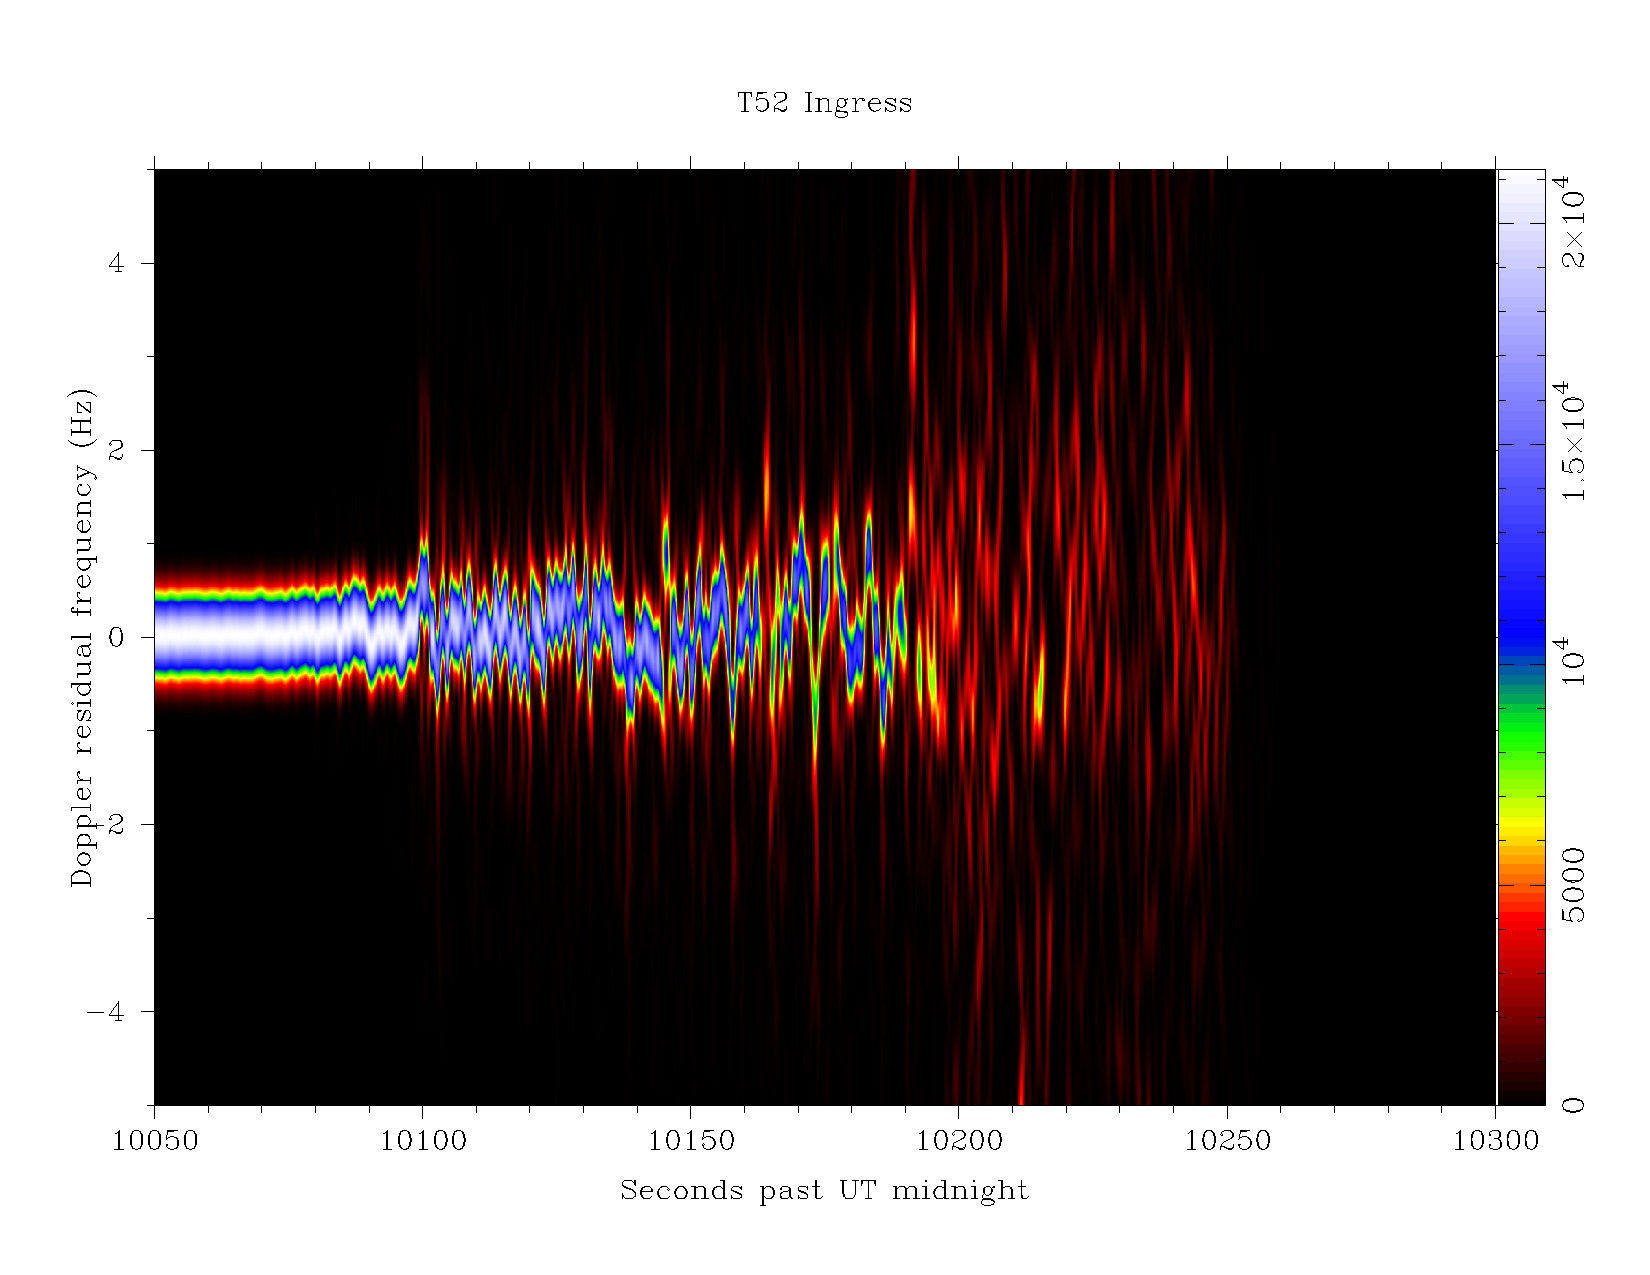
\includegraphics[page=1,width=3in]{non_copy.pdf}
            \hfill
            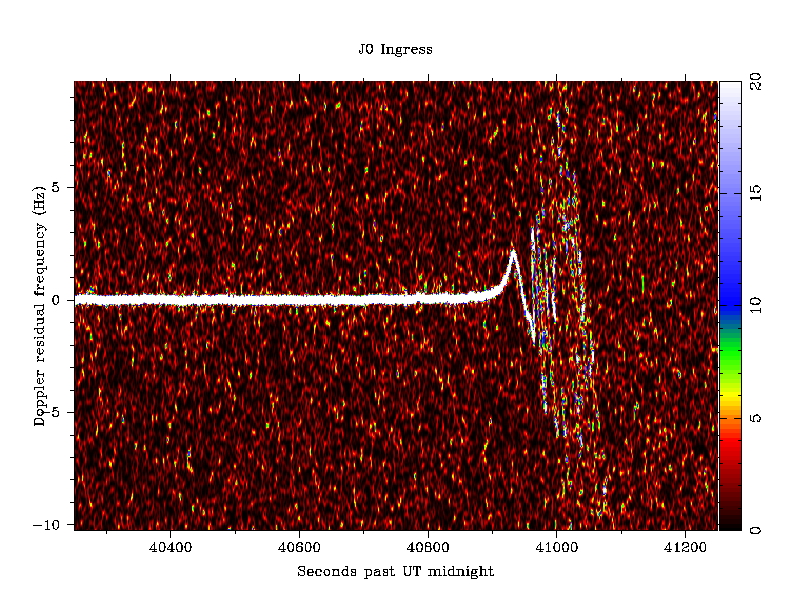
\includegraphics[width=3in]{non.png}
            \caption{Attachment from Paul Schinder}
        \end{figure}
        \subsubsection{\footnotesize RE: 1 KHz vs 16 KHz files}
        We're trying to finalize our data pipeline for ring analysis, and I still have some questions about the best way to extract power and phase at high time resolution (say, at 100 Hz). 
        \begin{enumerate}
            \item I had the naive idea that we ought to be able to get identical results when we analyze the 1 kHz files and the 16 kHz files, but I'm finding that the noise floor I derive for the 16 kHz files is larger than for the 1kHz files, which I'm not sure I understand. 
            \begin{itemize}
                \item Yes, you do get more noise because you’re using a wider bandwidth.  You’re not cutting off the noise above 500 Hz or below -500 Hz the way you do with 1 kHz.  You’ll see the same thing if you analyze 50 kHz or 100 kHz files. -Paul Schinder
            \end{itemize}
            \item Given a 1kHz and 16 kHz file from the same DSN for the same event, would you expect to get very similar/identical results from portspctrm for the two data files? If so, what changes to the input parameters would you need to make to ensure that equivalence (targeted to trying to get high time resolution for the derived power and phase).
            \begin{itemize}
                \item Yes, they should be very similar, but I don’t think you can ever guarantee they’re identical.  I just checked some files from S169 I have lying around and they’re within  mHz of each other when the signal is strong, but not identical. -Paul Schinder
            \end{itemize}
            \item For example, I analyzed the end of mission files with the command line parameters 1 1 1 (use 512 points per frequency point, skip 512 points per timestep) which at 1kHz gives a time resolution of 0.512 s.  If  we’d had 16 kHz and needed a better estimate of LOS, I probably would have used 8 1 1 (use 8*512 points, skip 512) which at 16 kHz is 0.512/16 s resolution, but with the caveat that there might be some unwanted correlations or smearing of the power drop off right at the end because of the chunking together of 8 * 512.  I’d probably pad that to get the frequency resolution up, too.
            \begin{itemize}
                \item Another question is this - does padding affect primarily the frequency resolution of your derived result (my supposition), or does it also affect the power estimation? -Paul Schinder
            \end{itemize}
        \end{enumerate}
        The intent is simply to increase the frequency resolution.  Since you’re adding zero power, it shouldn’t affect the power.  I’ll have to double check to make sure, though. -Richard French\par
        Thanks, Paul - we'll play around with this and see if we can make sense of it all. We are at the point now where we can get close to the same results that Essam gets for our estimates of power and phase, but we are not using any FFTs to do so - we are simply averaging the 1 kHz I and Q values and then taking $I^{2} + Q^{2}$ of the 0.25 km resolution sums for the power, and effectively atan(Q,I) for the phase, which we then adjust by removing the drift in frequency due to the imperfection of the predicts calculation. The problem with this approach is that the raw I and Q have noise in them that, for longer integration times, can be filtered out using FFT's by isolating the power peak in the FFTs, and getting a good frequency estimate from padding the FFT. Then the phase can in principle be recovered by integrating over $\delta freq\cdot dt$. What I'm trying to sort out is whether we can do better by using FFTs with the 16 kHz files to compute the power and frequency/phase at, say, 0.25 km resolution, than the method we are using now: just take the 1 kHz raw I and Q, compute $I^{2} + Q^{2}$ for power, atan(Q,I) for phase, and then correct for the phase drift with time of the predicts error. Our results in hand are not too bad, so if necessary we can proceed with our straightforward approach, but it relies on using the 1 kHz files at the moment, which are not part of the PDS archive. Ideally, we would use the 16 kHz files, even if computationally slower, so that we don't have to archive the 1 kHz RSR files, too. -Richard French
        \subsubsection{RE: SNR Ideas for the Record}
        \begin{enumerate}
            \item Write to Dick Simpson and Dave Hinson and ask them to compute thermal noise level for Rev007E 1 kHz file
            \item I think threshold optical depth is too optimistic - it accounts only for thermal noise, which applies only for the most opaque parts of the ring - and in any event our post-inversion profiles show a more realistic estimate of what the thermal noise actually is.
            \item For tenuous parts of the ring, such as the C ring, we care more about the minimum optical depth variation that we can believe in the data. For this, I think we can simply take the stdev of the normalized free-space signal (after inversion) at the actual spacing of the inverted profile (ex: 0.25 km for 1 km resolution data) and convert that to optical depth. That is a practical limit to the MINIMUM reliable optical depth variation. 
            \item Using this value, plot tau for the the tenuous regions of the C ring and Cassini Division on a scale where this minimum optical depth is plotted as a horizontal dashed line - it should pass through the excursions of the free-space signal.
            \item Another approach to estimating the limit of useful resolution is to determine the rms of the phase, in cycles, after removing the frequency offset, and finding the optical depth at which this rms phase exceeds 0.1 cycles. This should be a function of spatial resolution. Glenn can calculate this from the frequency-offset-corrected phase prior to inversion. An easy way to identify the limiting optical depth would be:
            \begin{itemize}
                \item plot rms of phase vs radius - there will be areas of opaque rings where this gets big and saturates.
                \item be aware that there will be blips where the rms phase will be artificially big because of phase wrapping, so plot as points instead of as lines, perhaps.
                \item plot tau vs radius on a separate panel
                \item plot rms of phase vs tau - there should be a trend of increasing rms with tau
                \item When rms of phase exceeds 0.1 cycle, this is a practical limit to the reliability of the phase evaluation and thus to the details of the ring structure at this resolution.
            \end{itemize}
        \end{enumerate}
        \subsubsection{\footnotesize RE: phase wrapping}
        Try running some intermediate cases of the number of points in the FFT: 2048, 4096, and 8192 come to mind as obvious possibilities. I expect that you'd see a trend in the magnitude of the difference in the phase shifts with the degree of averaging. I'm struck by the large DC phase shift, in addition to the slope that you demonstrate in the middle panel of plots - I would expect that this would increase rapidly with the amount of averaging, and it would be interesting to plot just that DC offset as a function of the number of points in the FFT divided by 1024, your base case. It might have some interesting curvature, and this is something that you could relate to the magnitude of the error in Simpson's rule, which is the method you are using for integration. Ryan would probably have some interest in predicting the error in Simpson's rule as you increase the step size, and seeing if your results agree. Similarly, if my hunch about the origin of the problem is right, you should find improvement as you successively increase the number of sub-points in your spline interpolation of the 16384 case from 2 to 16 (or perhaps even more).
        \subsubsection{\footnotesize RE: Phase Calculation to Try}
        I don't think we've yet tried an idea I had for computing the phase that might be more accurate than what we are doing now. Instead of using $phase = atan(\langle Q \rangle,\langle I \rangle)$, where the $\langle \rangle$ represents an average of measurements straight from the RSR (which I think is what we are doing now), the idea is that we use an analogous method to what we are doing when we compute power. 
        \begin{enumerate}
            \item Take the power spectrum of a small chunk of data - 16 points, I think, for 1KHz files.
            \item Find the location of the peak power and its adjacent m neighbors and add them up - that, I think is how we compute power now.
            \item Let those indices in the power spectrum that contribute to the power be an array L.
            \item Set all of the other elements in a copy of the FFT that produced the power spectrum to zero.
            \item Take the inverse FFT to reconstruct a time history of the reconstructed $I_r$ and $Q_r$ over those 16 points.
            \item Compute $\langle I_r\rangle^2 + \langle Q_r\rangle^2$ and compare it to the power you computed from the power spectrum itself - these should agree, perhaps to within a constant normalization factor.
            \item Compute $phase_{r} = atan(\langle Q_r\rangle ,\langle I_r \rangle)$ and compare to phase as computed above. 
            \item Try this for a variety of m neighbors.
        \end{enumerate}
        Ideally, this would give good agreement where the signal is strong, but give improved results where the signal is weaker, as in the center of an opaque ring. Would you make a plot of the results for the Maxwell Ringlet and Huygens Ringlet, to see if this works at all? (For starters, you can do this just for the I and Q without having to apply the frequency offset part, unless it's just as easy to do the entire process to compute the final phase.) Compare the results to our previous method for both phase and power, and to Essam's from the savefile that gives the pre-Fresnel-inversion phase and power. Then make a final set of plots to compare the methods and make a decision about which method is best for computing the phase. If so, then let's use this method to compute the phase for the full. Rev007E to confirm that it works.
        \subsection{To Do List}
            \begin{enumerate}
                \item Talk about processing pipeline.
                \begin{itemize}
                    \item Geometry
                    \begin{itemize}
                        \item Mindfully choose the RSR you want.
                              Radial coverage, opening angle, etc.
                    \end{itemize}
                    \item Phase and power retreival
                    \begin{itemize}
                        \item Picking start and end SPM
                        \item Choosing nots
                        \item Choosing order of residual frequency fit
                    \end{itemize}
                    \item Diffraction reconstruction
                    \begin{itemize}
                        \item Choose resolution, window type, and range.
                    \end{itemize}
                    \item Look at Essam's new directory structure.
                    \item Look at Essam's diffraction profiles. Try to recreate his corrected profiles using the diffraction reconstruction code.
                \end{itemize}
                \item Document the ideal, or optimal, resolution
                      to compare
                      with Essam based on comparisons with $L_{1}$,
                      $L_{2}$, and $L_{\infty}$ for various revs,
                      including
                      old high resolution data sets from various idl .sav
                      files. Include documentation on the effect of using
                      different windows for these comparisons. Show that
                      the best match uses a window (KBMD20) that is not
                      mentioned in MTR86.
                \item Document what v2 diffraction reconstruction did.
                      npoints parameter for FFT. etc.
                \item Look for waves in the D ring to compare
                      with VIMs data.
                      If these are dusty rings, the radio data shouldn't
                      see it. Range 73000 to inner C ring. Compare with
                      Colleen's results.
                \item Essam assumes uniform power across rings,
                      but there is
                      an antenna beam patter. Learn about this. Try this
                      problem on a square well.
                      The wave is a sinc function
                      in terms of the angle from the on-axis ray.
                      The first null is proportional to
                      $\lambda/d$, where
                      $d$ is the antenna diameter. Ask prof French about
                      more accurate numbers and models.
                \item Document disk swapping in Rev133. In Unix: ps au.
                      Document variations in points processed per second.
                      Note is should decrease with window size, but
                      doesn't.
                \item Document the differences in v4 and v5.
                \item Add these regions (Try finding waves):
                \begin{itemize}
                    \item Mi 4:1 m=2  74890 km  1.1$\pm$0.5 g/$\textrm{cm}^2$  0.16$\pm$0.09  0.18$\pm$0.13 g/$\textrm{cm}^2$
                    \item W74.66 m=-7 74666 km  0.7$\pm$0.2 g/$\textrm{cm}^2$  0.09$\pm$0.03  0.15$\pm$0.09 g/$\textrm{cm}^2$
                    \item W74.93 m=-4 74936 km  0.3$\pm$0.1 g/$\textrm{cm}^2$  0.05$\pm$0.02  0.21$\pm$0.17 g/$\textrm{cm}^2$
                    \item W74.94 m=-9 74941km,  1.3$\pm$0.5 g/$\textrm{cm}^2$, 0.17$\pm$0.07  0.14$\pm$0.07 g$\textrm{cm}^2$
                    \item W76.02 m=-9 76018km,  1.3$\pm$0.7 g/$\textrm{cm}^2$, 0.05$\pm$0.04  0.05$\pm$0.05 g$\textrm{cm}^2$
                    \item W76.23 m=-8 76237.5km 1.6$\pm$1.0 g/$\textrm{cm}^2$, 0.17$\pm$0.06  0.15$\pm$0.09 g$\textrm{cm}^2$
                    \item W76.44 m=-2 76435.5km 1.0$\pm$1.4 g/$\textrm{cm}^2$, 0.04$\pm$0.02  0.07$\pm$0.05 g$\textrm{cm}^2$
                \end{itemize}
                \begin{itemize}
                    \begin{multicols}{2}
                        \item Kuiper Gap 119400 $\pm$30km
                        \item Jeffreys Gap 118950 $\pm$40km
                        \item Russell gap 118610 $\pm$40km
                        \item Bessel-Barnard 120270 $\pm$50km
                        \item Strange Ringlet 117910 $\pm$30km
                        \item Herschel Gap 118240 $\pm$140km
                    \end{multicols}
                \end{itemize}
            \end{enumerate}
\end{document}